%\documentclass[wcp,gray]{jmlr} % test grayscale version
\documentclass[wcp]{jmlr}% former name JMLR W\&CP
%\documentclass[pmlr]{jmlr}% new name PMLR (Proceedings of Machine Learning)

 % The following packages will be automatically loaded:
 % amsmath, amssymb, natbib, graphicx, url, algorithm2e
 \usepackage{amsmath,amssymb,graphicx,url}

 %\usepackage{rotating}% for sideways figures and tables
\usepackage{longtable}% for long tables

 % The booktabs package is used by this sample document
 % (it provides \toprule, \midrule and \bottomrule).
 % Remove the next line if you don't require it.
\usepackage{booktabs}
 % The siunitx package is used by this sample document
 % to align numbers in a column by their decimal point.
 % Remove the next line if you don't require it.
\usepackage[load-configurations=version-1]{siunitx} % newer version
 %\usepackage{siunitx}

% Package to make table with multi rows and columns
\usepackage{multirow}
 
 % to do
\usepackage{xcolor}
\newcommand\todo[1]{\textcolor{red}{#1}}

 % change the arguments, as appropriate, in the following:
\jmlrvolume{}
\jmlryear{}
\jmlrworkshop{STA723 -- Case Study 1}
\jmlrproceedings{}{}


% start article
% \titlebreak
% \footnote{}
% \textsf

\title[DDE and PCB effect on Premature delivery]{Assessing Effects of Exposures to DDE and PCBs on Premature Delivery via Ordinal Logistic Regression}	%\titletag{\thanks{XXX}} % leave empty?

 % Use \Name{Author Name} to specify the name.
 % If the surname contains spaces, enclose the surname
 % in braces, e.g. \Name{John {Smith Jones}} similarly
 % if the name has a "von" part, e.g \Name{Jane {de Winter}}.
 % If the first letter in the forenames is a diacritic
 % enclose the diacritic in braces, e.g. \Name{{\'E}louise Smith}

 % Authors with different addresses:
 
 \author[Morsomme, Ou, Zito]{Raphael Morsomme \and Rihui Ou \and Alessandro Zito}
 \date{\today} % Date, can be changed to a custom date
 
 % Three or more authors with the same address:
 % \author{\Name{Author Name1} \Email{an1@sample.com}\\
 %  \Name{Author Name2} \Email{an2@sample.com}\\
 %  \Name{Author Name3} \Email{an3@sample.com}\\
 %  \addr Address}

 % Authors with different addresses:
 % \author{\Name{Author Name1} \Email{abc@sample.com}\\
 % \addr Address 1
 % \AND
 % \Name{Author Name2} \Email{xyz@sample.com}\\
 % \addr Address 2
 %}

% leave editor's section empty?
%\editor{Editor's name}
% \editors{List of editors' names}

\begin{document}

\maketitle

%\begin{abstract} \end{abstract}

\section{Introduction}
\label{sec:intro}

Dichlorodiphenyldichloroethylene (DDE) and Polychlorinated Biphenyls (PCB) are two chemical elements which were commonly in use in the United States for agricultural purpouses and were banned during the 70's due to their detrimental effect on human health. Exposure to these chemical products has been linked to neurobehavioral and developmental deficits in newborns. As the human body stores them in its fatty tissues, studying their impact on human health is particularly important.

In this report, we examine the effect of DDE and PCB on fetuses; more precisely, we assess the potential association between the exposure to these chemicals and the chance of early delivery. Ideally, a higher exposure to the substances induces a preterm delivery, which may have adverse consequences for the child. To verify this theory, we construct an ordinal logistic regression model over three delivery groups  We find that the impact of the substances is essentially race specific: exposure to DDE increases the risk of early childbirth among white people and exposure to PCB increases the risk among non-white ones. 

The report is divided as follows: \sectionref{sec:data} describes the data, \sectionref{sec:method} presents our methodology,  \sectionref{sec:results} reports our findings, \sectionref{sec:conclusion} discusses the results and concludes.

\section{Data}
\label{sec:data}
The data set consists of 2,380 pregnant women that visited a hospital during their pregnancy in 2001. It contains the length of the gestation in weeks, the concentration doses of DDE and the twelve PCB breakdown products in the blood, the concentration of cholesterol and triglycerides and several demographic information (race, level of education, income, occupation, age, smoking status and the center attended by the woman).

 The data were not clean. In particular, 43 women showed a length of gestation superior to 45 weeks (the second longest gestation period ever recorded), and 1 women did not show any records of the PCBs levels. Thus, we decide to drop them, reducing the observations to 2,336. Finally, we mean impute the missing data on the income, education and occupational scores\footnote{Note that these scores will not end up in the final model.}


\section{Method}
\label{sec:method}
As a first step, we divide the 
\subsection{Feature Engineering}
First, since we focus on the impact of DDE and PCB on early delivery, we dichotomize the dependent variable \textit{gestational duration} measured in weeks into three levels: at risk for gestation shorter than $33$ weeks, pre term for gestation between $34$ and $36$ week, and at term for gestation longer than $37$ weeks. 
Second, we also aggregate the 12 PCB measurement into one variable since these variables are highly correlated (see \figureref{fig:corr}). To accomplish this, we take their average after standardizing them in order to prevent one measurement to dominate the aggregate variable. 
Third, we combine the measurements of chemical in blood with the fat-related variables to estimate the level chemical to which the women were exposed. We start by estimating the total amount of fatty tissues using the following formula (\todo{reference})

\begin{equation}
\label{eq:fat}
\text{lipid} = 2.27 * \text{cholesterol} + \text{triglycerides} + 0.623.
\end{equation}
Since the amount of chemical absorbed is proportional to the amount of fatty tissue one has, we divide the concentration of PCB and DDE in blood by the estimated amount of fatty tissue in order to obtain an estimate of the initial level of exposure to these chemical product, that is,
\begin{equation}
\label{eq:exp_dde}
\text{DDE}_{\text{exposure}} = \dfrac{\text{DDE}}{\text{lipid}}
\end{equation}
and 
\begin{equation}
\label{eq:exp_pcb}
\text{PCB}_{\text{exposure}} = \dfrac{\text{PCB}_\text{aggregate}}{\text{lipid}}.
\end{equation}

Finally, we combine \textit{black} ($n=??)$ and \textit{other} ($n=??$) in the variable \textit{race} in order to have levels with a sufficient amount of data.

\begin{figure}[htbp]
	\floatconts
	{fig:corr}
	{\caption{Correlation among the 12 PCBs variables.}}
	{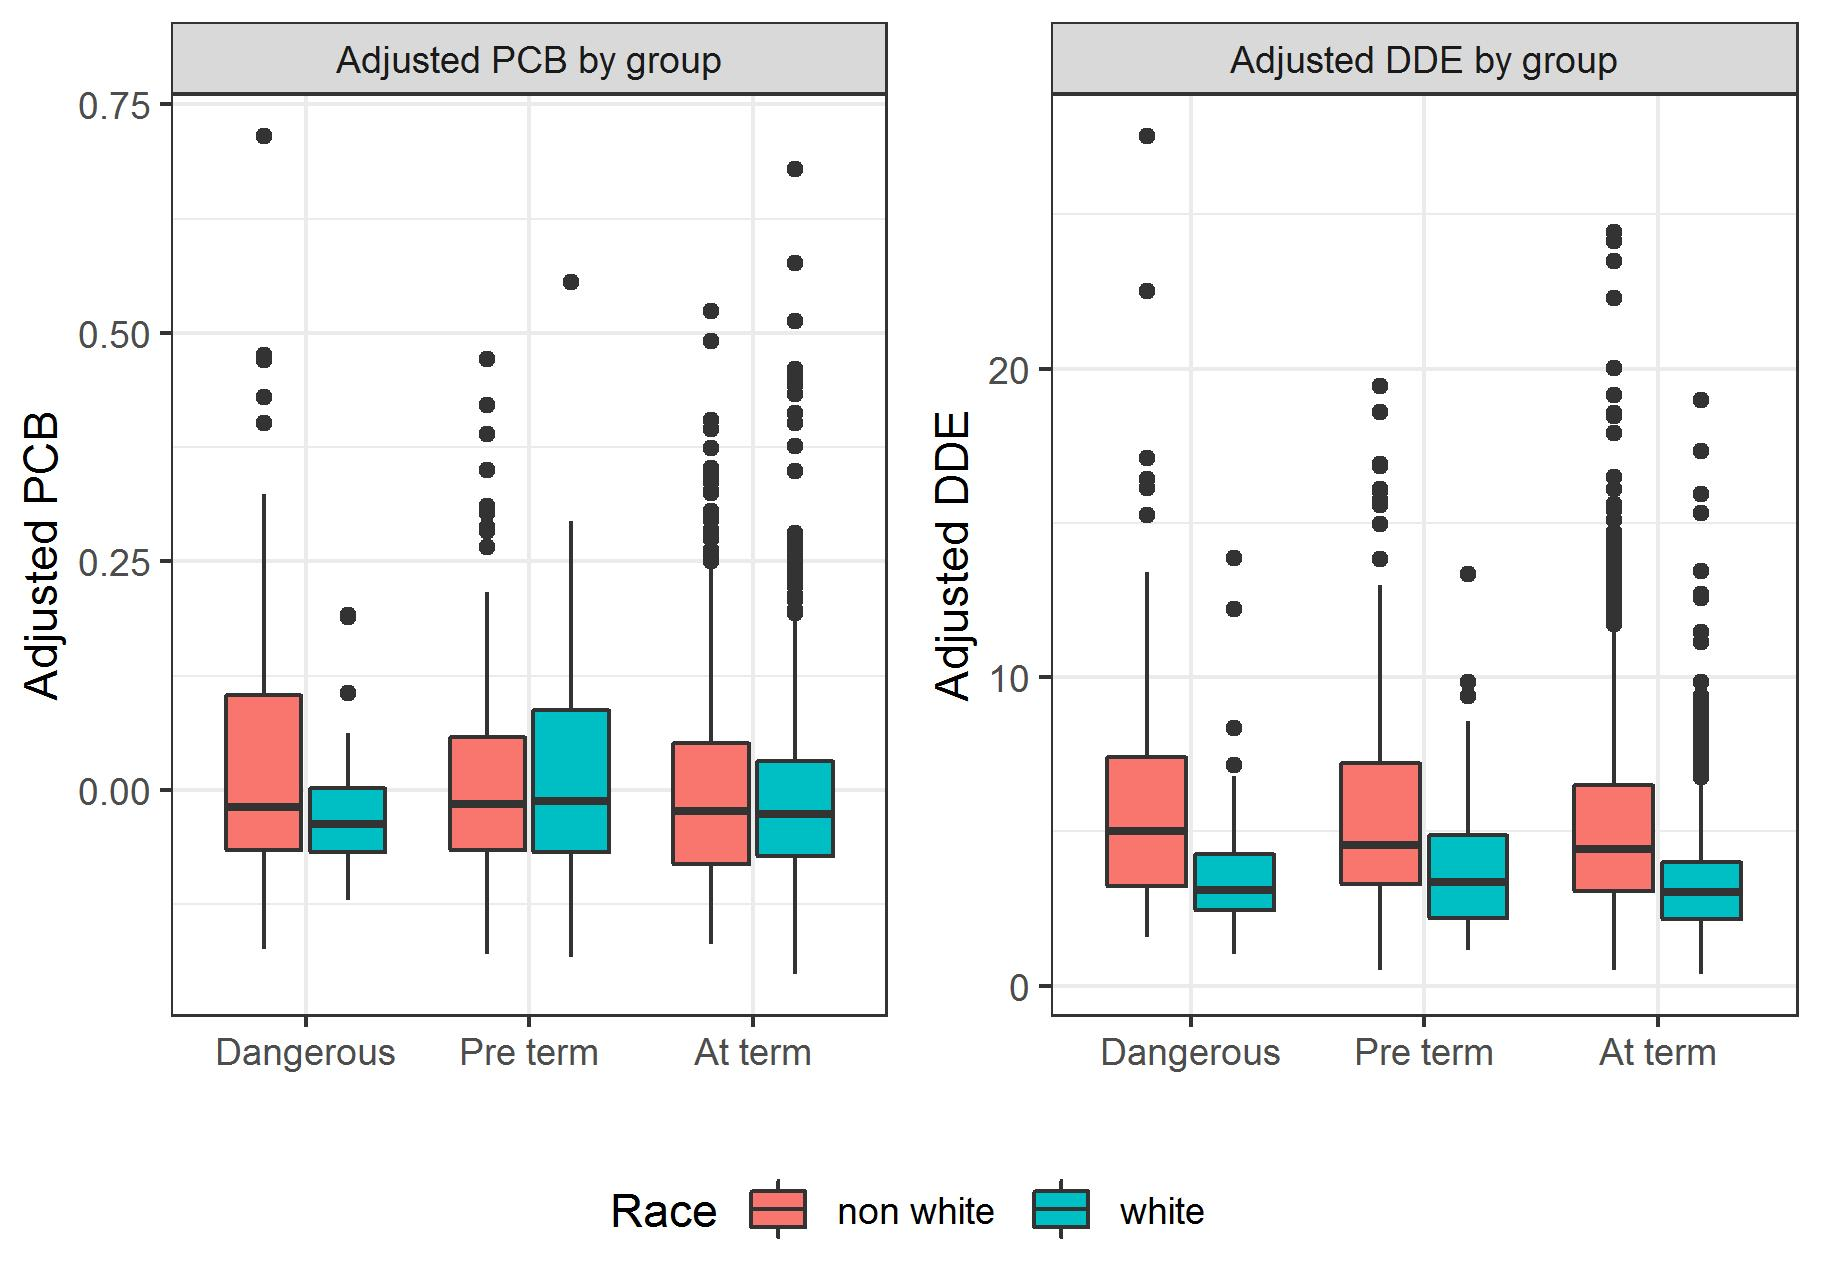
\includegraphics[width=0.8\linewidth]{pcb_corr}}
\end{figure}

\subsection{Ordinal Logistic Regression Model}
$\text{DDE}_{\text{exposure}}$ and $\text{¨CB}_{\text{exposure}}$ are the variables of interest. In order to identify non-spurious association between these variable and the occurrence of early deliveries, we control for $7$ background attributes: \todo{list them}.
\todo{interaction with centers and race to allow different effect across centers and race}

Since not all attributes are necessarily related to the dependent variable, we conduct an backward AIC-based variable selection procedure. Ideally, we would have preferred to avoid selecting variables and instead run a BMA, but since Merlise's package does not allow ordinal logistic regression, we opted for the simpler frequentist approach. The variable selection procedure includes \todo{list variables} and drops \todo{list variables}.

We use the variables selected y the procedure as predictors in a Bayesian ordinal logistic regression model. The model was fit using stan. We use $10$ chains of $10,000$ iterations each, and put a uniform prior on the coefficients.




\begin{table}[hbtp]
	\floatconts
	{tab:student-data}
	{\caption{Example of student data}}	
	{\begin{tabular}{ccccc}
		\toprule
		\bfseries Student ID &\bfseries Course ID &\bfseries Academic Year &\bfseries Period &\bfseries Grade\\
		\midrule
		44940 & CAP3000 & 2009-2010 & 4 & 8.8\\
		37490 & SSC2037 & 2009-2010 & 4 & 8.4\\
		71216 & HUM1003 & 2010-2011 & 4 & 6.8\\
		44212 & SSC2049 & 2010-2011 & 2 & 8.4\\
		85930 & SSC2043 & 2011-2012 & 1 & 4.3\\
		\addlinespace
		14492 & COR1004 & 2012-2013 & 2 & 8.5\\
		34750 & HUM2049 & 2013-2014 & 5 & 6.0\\
		32316 & SSC1001 & 2013-2014 & 1 & 8.5\\
		22092 & SCI1009 & 2014-2015 & 1 & 6.4\\
		19512 & COR1004 & 2016-2017 & 5 & 7.0\\
		\bottomrule
	\end{tabular}}	
\end{table}


\section{Results}
\label{sec:results}

Main findings: the effect of the chemicals on the risk of early delivery is race dependent. Exposure to DDE has a particularly detrimental impact on the gestation process among white women, while exposure to PCB affects non-white more (see \figureref{fig:results})).


\begin{figure}[htbp]
	\floatconts
	{fig:corr}
	{\caption{Estimated probability of gestation outcomes in function of race, and exposure to DDE and PCB.}}
	{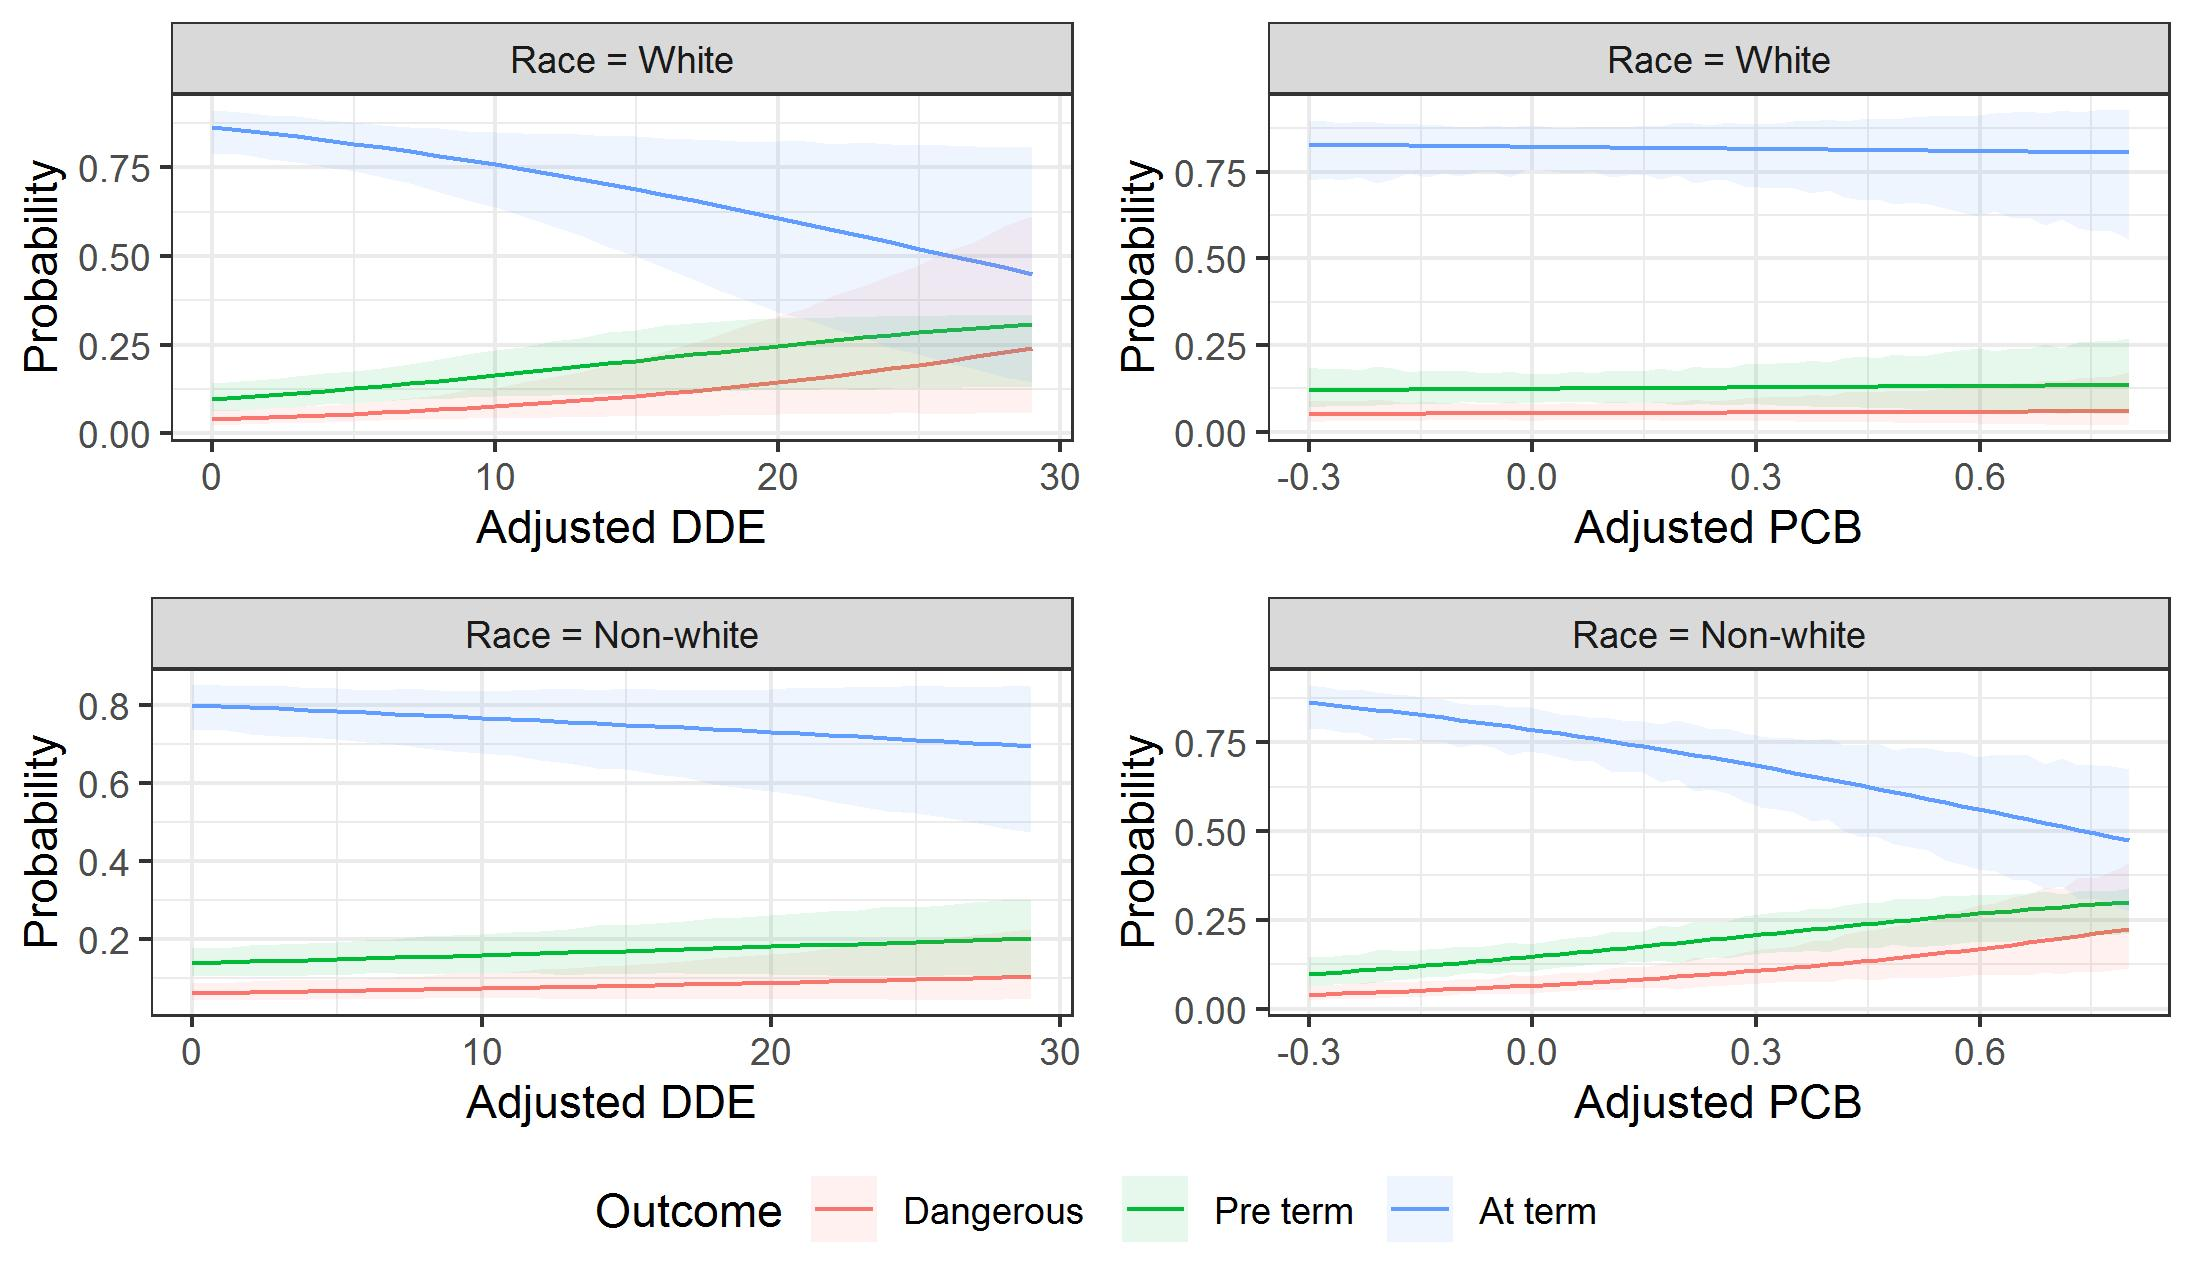
\includegraphics[width=0.8\linewidth]{results}}
\end{figure}



\section{Conclusion}
\label{sec:conclusion}

Future, add quadratic term to age since gestations at a young and an old age are more at risk of complications.

Consider interaction between PCB and DDE

%\bibliography{bibliography}

\end{document}